\paragraph{Co działa, a co nie.}
\begin{itemize}
  \item \textbf{ArcFace} daje największy pojedynczy zysk tam, gdzie baseline był najsłabszy:
        Rank-1 GRU na dev rośnie z 0{,}820 do 0{,}979, a EER spada ponad trzykrotnie. Usunięcie ArcFace z
        pełnego przepisu (CE zamiast ArcFace) cofa GRU do 0{,}907 (tab.~\ref{tab:sota-extra}).
        Dla Transformera i InceptionTime zysk wynosi ok.~1~p.p., a dla ResNet1D jest w granicach
        szumu.
  \item \textbf{Prędkości} to drugi kluczowy składnik. Poprawiają \emph{wszystkie} cztery modele
        (ResNet1D 0{,}945~$\to$~0{,}975, Transformer 0{,}967~$\to$~0{,}982) i obniżają EER do
        ok.~0{,}010--0{,}014. Pierwsza różnica jest niezmiennicza względem stałego przesunięcia, więc
        uwypukla dynamikę ruchu, która jest stabilniejsza między dniami niż położenie.
  \item \textbf{Augmentacje, EMA i centrowanie poziome} nie dały mierzalnego zysku: zmiany mieszczą
        się w $\pm 1{,}5$~p.p., czyli do ok.~9 prób z 615 na dev (dla ResNet1D augmentacje nawet
        nieco szkodzą), a usunięcie augmentacji lub centrowania z pełnego przepisu niczego nie
        pogarsza. Zostawiamy je w przepisie, bo tak został wybrany, ale
        uczciwie raportujemy, że nie są źródłem poprawy.
  \item \textbf{Trening na całym dniu~1} poprawił dev dla obu sprawdzonych modeli (GRU
        0{,}984~$\to$~0{,}987, Transformer 0{,}982~$\to$~0{,}985), dlatego jest częścią przepisu
        finalnego. Pozostałe warianty (margines 0{,}5, skala 64, 250 epok) nie dały spójnej poprawy
        Rank-1 na obu modelach.
\end{itemize}

\paragraph{Wynik końcowy.} Przepis \emph{pełny + trening na całym dniu~1} uruchomiliśmy dla 4 modeli i
3 seedów (42, 43, 44). Ensemble wszystkich czterech modeli wybraliśmy na dev (0{,}992 wobec 0{,}991
bez GRU). Wyniki zawiera tabela~\ref{tab:sota-final}.

\begin{table}[H]
\centering\footnotesize
\setlength{\tabcolsep}{2.2pt}
\caption{S4: wynik końcowy, średnia $\pm$ odch. std. z 3 seedów. \emph{Test} -- dzień 2, rzuty 5--9,
niewidziane przy żadnej decyzji (wynik główny). Kolumna S2 -- baseline (pełny, 3 seedy) na całym
dniu 2. Galerią w S4 jest cały dzień 1.}
\label{tab:sota-final}
\begin{tabular}{@{}lrrrrrrrr@{}}
\toprule
& S2 & cały dz. 2 & \multicolumn{3}{c}{Test (dzień 2, rzuty 5--9)} & \multicolumn{3}{c}{Test: R-1 wg urządz.} \\
\cmidrule(lr){3-3}\cmidrule(lr){4-6}\cmidrule(l){7-9}
Model & Rank-1 & Rank-1 & Rank-1 & Rank-5 & EER & Quest & Vive & Cosmos \\
\midrule
\tabinput{tables/sota_final.tex}
\bottomrule
\end{tabular}
\end{table}

\begin{figure}[H]
\centering
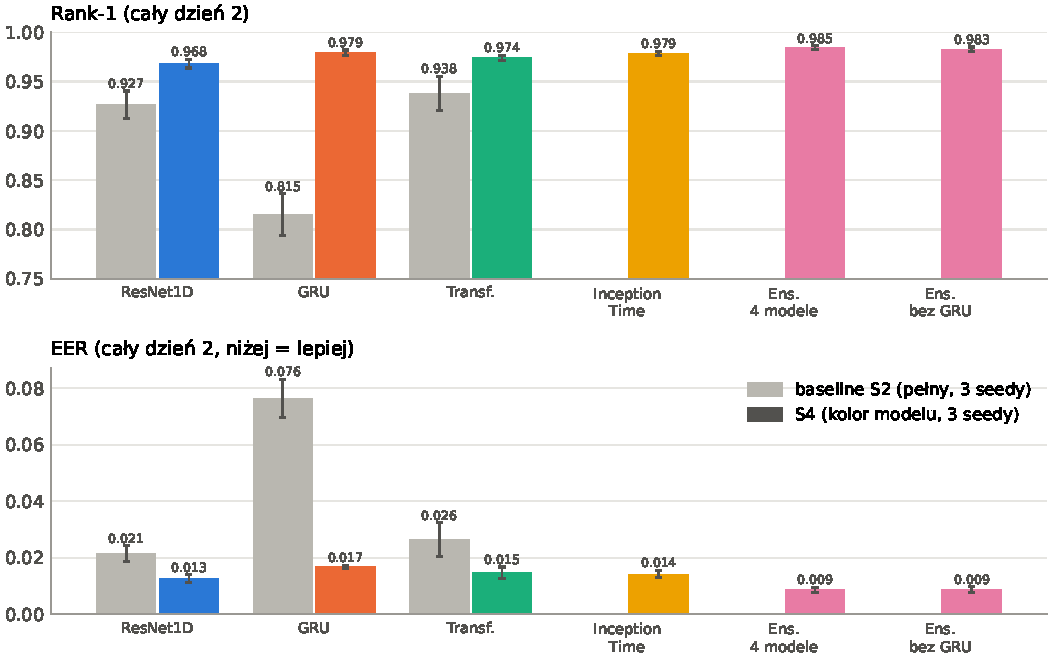
\includegraphics[width=\linewidth]{sota_vs_baseline.pdf}
\caption{S4 a baseline z S2 na całym dniu 2 (średnia $\pm$ odch. std. z 3 seedów). InceptionTime i
ensemble nie mają odpowiednika w S2.}
\label{fig:sota-vs-base}
\end{figure}

\begin{itemize}
  \item \textbf{Ensemble 4 modeli: Rank-1 $0{,}977 \pm 0{,}002$ i EER $0{,}012$ na odłożonym teście}
        (na całym dniu~2: 0{,}985 i 0{,}009). Najlepszy baseline (Transformer, 0{,}938) mylił się w
        6{,}2\% prób dnia~2, a ensemble w 1{,}5\%, czyli ok.~4 razy rzadziej. EER spadł z 0{,}021
        (najlepszy w S2) do 0{,}009.
  \item \textbf{Pojedyncze modele zbliżyły się do siebie.} Na teście wszystkie cztery mieszczą się w
        przedziale 0{,}960--0{,}972. GRU, najsłabszy w S1--S2 (0{,}815), w S4 jest wśród najlepszych
        (0{,}971): jego słabość wynikała z funkcji straty i cech wejściowych, a nie z architektury.
        Najlepszym pojedynczym modelem jest InceptionTime (0{,}972), a najniższy EER ma ResNet1D
        (0{,}016).
  \item \textbf{Geometria embeddingów:} ArcFace przesuwa pary impostor do podobieństwa ok.~0
        (ortogonalne embeddingi; w S1 było 0{,}28--0{,}47), co dobrze widać na rozkładach
        (rys.~\ref{fig:scores-sota}).
  \item \textbf{Cosmos nadal najtrudniejszy:} 0{,}93--0{,}94 Rank-1 wobec 0{,}97--1{,}00 dla Questa i
        Vive. W teście ensemble ok.~85\% pozostałych błędów (średnio 12 z 14) to próby z Cosmosa.
  \item \textbf{Optymizm dev.} Na dev ensemble osiąga 0{,}992, na teście 0{,}977. Na modelach z S1,
        które dev nigdy nie widziały, obie połowy dnia~2 są równie trudne (różnice $\pm$1~p.p. bez
        stałego kierunku), więc ok.~1~p.p. różnicy to koszt wyboru przepisu na dev. Właśnie dlatego
        jako wynik główny podajemy odłożony test.
\end{itemize}

\begin{figure}[H]
\centering
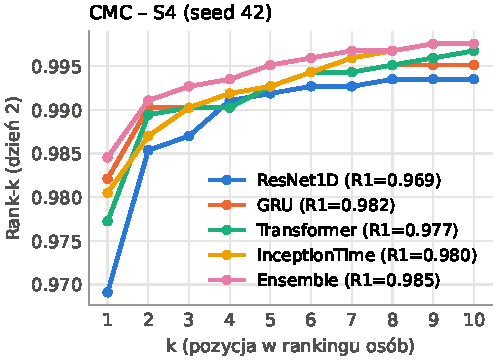
\includegraphics[width=0.55\linewidth]{cmc_sota.pdf}
\caption{S4: krzywe CMC na całym dniu 2 (seed 42). Ensemble: Rank-1 0{,}985, Rank-5 0{,}995.}
\label{fig:cmc-sota}
\end{figure}

\begin{figure}[H]
\centering
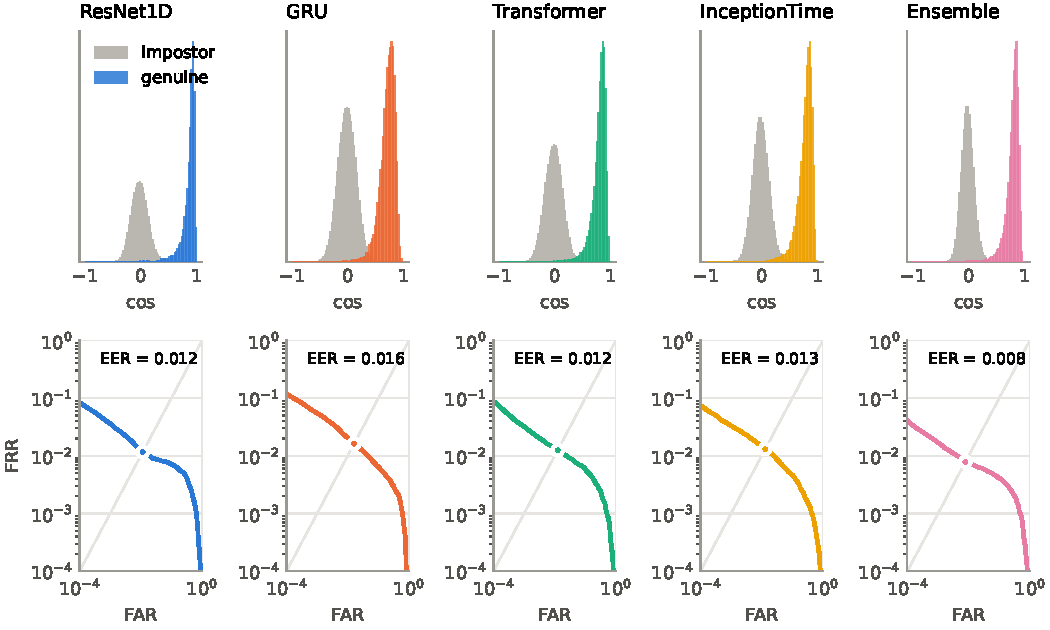
\includegraphics[width=\linewidth]{scores_sota.pdf}
\caption{S4: rozkłady podobieństwa genuine/impostor i krzywe DET (cały dzień 2, seed 42).
W porównaniu z rys.~\ref{fig:scores-base} rozkład impostor przesunął się do zera, a krzywe DET
leżą niżej.}
\label{fig:scores-sota}
\end{figure}
